\chapter{Elektronische Transporteigenschaften}

Bewegung der \(e^-\)-nen, effektive Masse.

\section{Elektronien als Wellenpakete}

Ausgedehnte Wellen \(\delta k\delta r > 1\)

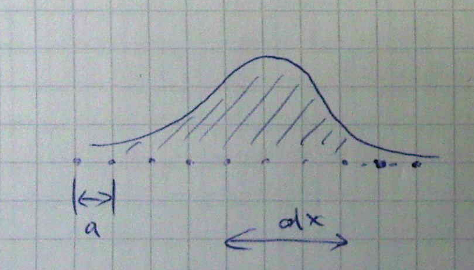
\includegraphics[width=0.75\textwidth]{kap10_01.png}

\[\psi(\vec r,t) = \sum_{\vec k} g(\vec k)\cdot e^{i(\vec k\vec r - \frac{\hbar k^2}{2m}t}\]

mit \(r= \frac{pt}{2m}\)

Koeffizienten \(g(\vec k)\) sind innerhalb \(\delta k\) 'gaußförmig' verteilt. Das entspricht einer semiklassischen Näherung. 

\[\frac{\partial \vec r}{\partial t} \equiv \vec v(\vec k) = \frac{1}{\hbar}\nabla_{\vec k}E(\vec k) = \frac{1}{\hbar} \frac{\partial E(\vec k)}{\partial \vec k} \]

mit \(E(\vec k) \) Energie vom Wellenpaket. z.B. für freie \(e^-\)-nen \(E=\frac{\hbar^2 k^2}{2m}\); \(v_g=\frac{\hbar k}{m}\) Gruppengeschwindikeit.

Semiklassische Bewegungsgleichung:

\[\hbar \frac{\partial \vec k}{\partial t}=\vec F = -e\vec \vec{ \mathcal E}(\vec r,t) -\vec v(\vec k)\times \vec B(\vec r,t)  \]

\(\vec{ \mathcal E}\) Elektrisches Feld; \(\vec B\) magnetisches Feld; \(E(\vec k) = E(-\vec k)\)

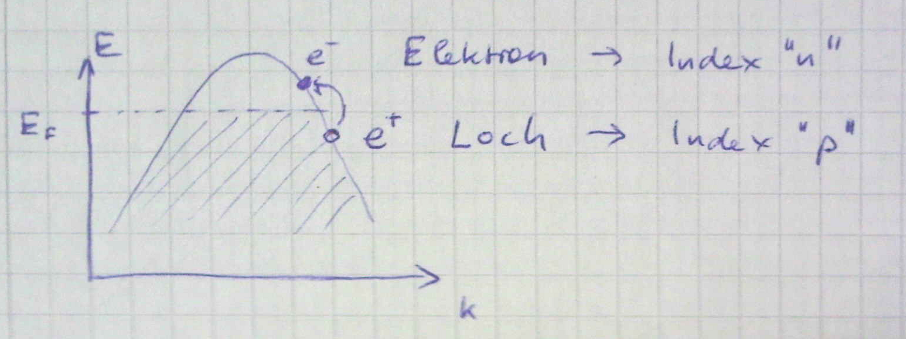
\includegraphics[width=0.75\textwidth]{kap10_02.png}

\(E_p(\vec k) = -E_n(\vec k)\); \(\sum \vec k = 0\); \(\vec k_p = - \vec k_n \)

Gruppengeschwindigkeit: \(\frac{\partial \vec v}{\vec t}(\frac{1}{\hbar}\frac{\partial E(\vec k)}{\partial \vec k})=\frac{\partial}{\partial \vec k}(\frac{1}{\hbar}\frac{\partial E(\vec k)}{\partial \vec k})\frac{d\vec k}{dt}=\frac{1}{\hbar^2}\vec F\frac{\partial^2 E(\vec k}{\partial \vec k\partial\vec k}\)

\[\frac{\partial v_i}{\partial t} = \frac{1}{\hbar}\sum_j \frac{\partial^2 E(\vec k)}{\partial k_i\partial_j}F_j\]

Tensor der effektive Masse \([m*]\equiv \stackrel{\mathrm{=}}m^* \)

mit 

\[\left(\frac{1}{m^*}\right)_{ij}=\frac{1}{\hbar^2}\frac{\partial^2 E(\vec k)}{\partial k_i\partial k_j}\]


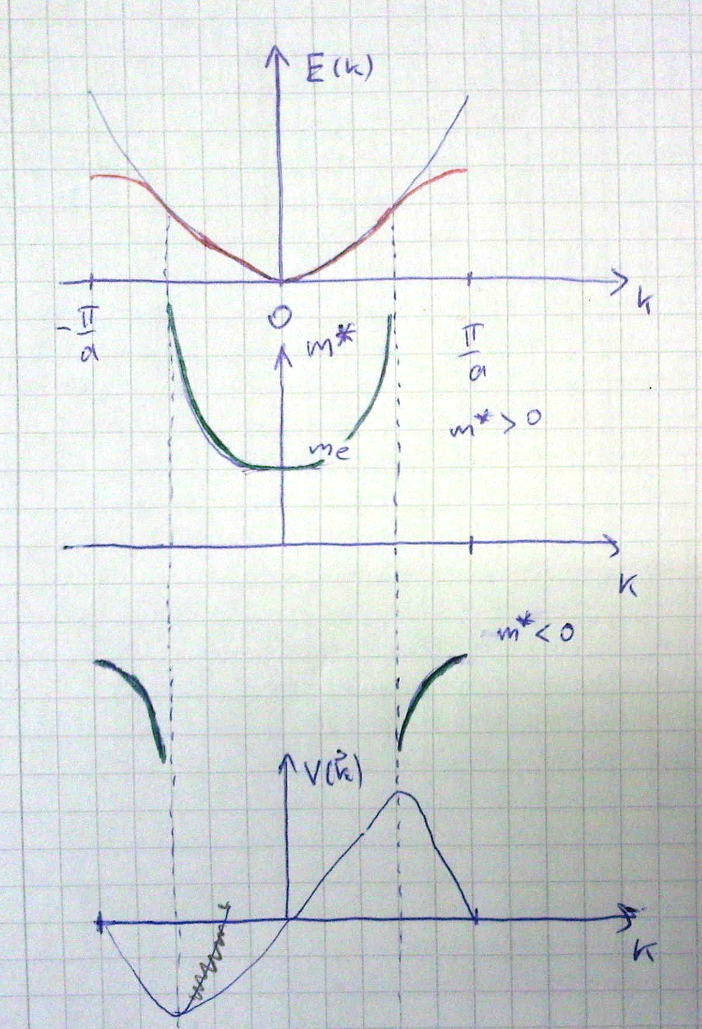
\includegraphics[width=0.75\textwidth]{kap10_03.png}

1D: \(m^*\) ist klalare Größe \(m^*(k) = \frac{\hbar^2}{[\frac{d^2E(k)}{dk^2}]}\)

Bloch-oszillationen: \(\hbar \frac{dk}{dt} = F = -e\mathcal E\)


Periode dieser Bloch Oszillationen:

\[T\propto \frac{\delta k}{|dk/dt|}\propto \frac{2\pi/a}{e\mathcal E/\hbar}\]


\section{Ladungstransport: Elektronen und Löcher}

\[\left[\frac{1}{m^*}\right]_{p}=\frac{1}{\hbar^2}\left[\frac{\partial^2 E(\vec k)}{\partial \vec k\partial \vec k}\right]_{p}=\frac{1}{\hbar^2}\left[\frac{-\partial^2 E(\vec k)}{(-\partial \vec k)(-\partial \vec k}\right]_{p} = -\left[\frac{1}{m^*}\right]_n \]


Bewegungsgleichungen: 

\[\hbar \frac{\partial \vec k_n}{\partial t} = -e(\mathcal{\vec E} + \vec v_n\times\vec B)\]
\[\hbar \frac{\partial \vec k_p}{\partial t} = +e(\mathcal {\vec E} + \vec v_p\times\vec B)\]


\section{Elektronen im Magnetfeld}

Semiklassische Näherung für Bloch Elektronen

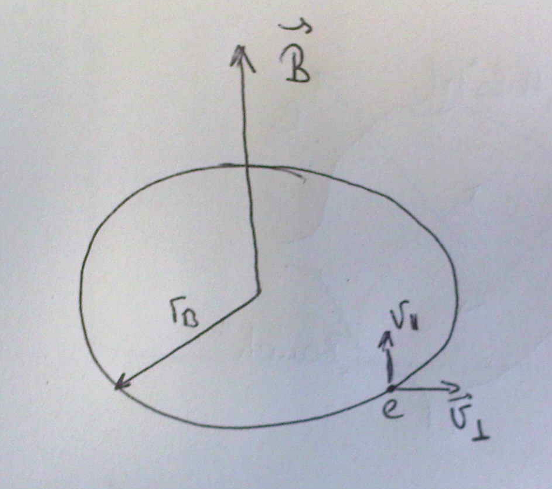
\includegraphics[width=0.75\textwidth]{kap10_04.png}

Im realen Raum: \(\tau_B = \frac{m v_\bot}{eB}\)
Umlauffrequenz ist Zyklotronfrequenz: \(\omega_c = \frac{eB}{m}\)
Im \(\vec k\)-Raum mit \(\vec v = \frac{1}{\hbar }\frac{\partial E}{\partial \vec k}\), und \(\hbar \frac{\partial \vec k}{\partial t} = \vec F\)
durch \(E=const\), \(\Rightarrow \frac{\partial E}{\partial t} = \frac{\partial E}{\partial \vec k}\cdot\frac{\partial \vec k}{\partial t} = \hbar\vec v ( - \frac{e}{\hbar}\vec v \times\vec B) = 0\)

durch \(k_n=const\), \(\Rightarrow \frac{\partial(\vec k\cdot\vec B}{\partial t} = \frac{\partial \vec k}{\partial t}\cdot \vec B + \frac{\partial \vec B}{\partial t}\cdot\vec k = 0\)

Im \(\vec k\)-Raum Umlaufbahn eines Elektron ist eine Schnittlinie von eine Fläche konstanter Energie ( \(\equiv\) Fermi-Fläche \(T<<T_F\) und eine Ebene \(\bot \vec B\) (\(\vec k_{||} = const.\))

\begin{enumerate}
\item[a)] 'geschlossene' Fermi-Fläche
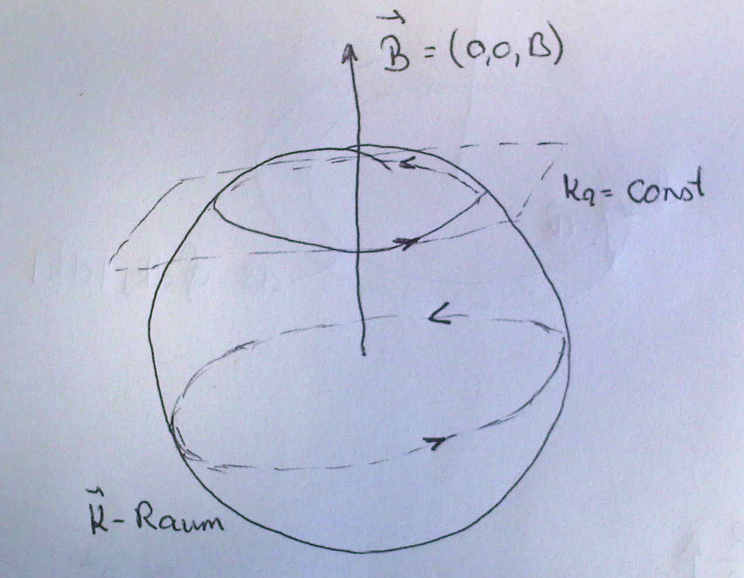
\includegraphics[width=0.75\textwidth]{kap10_05.png}

\item[b)] 'Offene' Fermi-Fläche (z.B. Cu,Au)
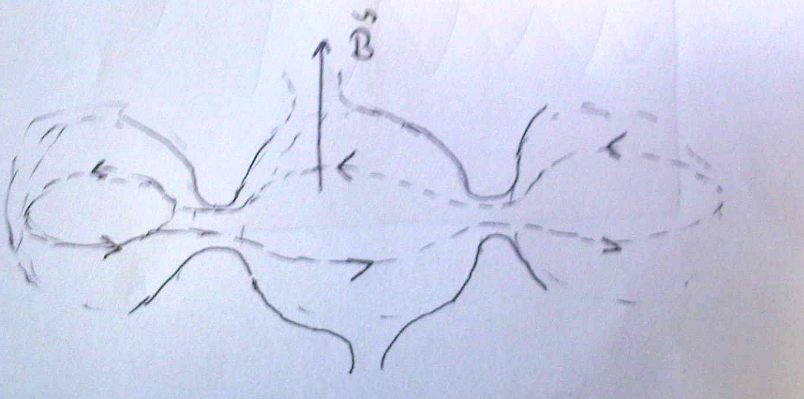
\includegraphics[width=0.75\textwidth]{kap10_06.png}
\end{enumerate}


Bewegungsrichtung: \(\frac{\partial \vec k}{\partial t} = -\frac{e}{\hbar}\vec v \times \vec B = -\frac{e}{\hbar^2}\frac{\partial E}{\partial \vec k}\times \vec B\)

Die Zeit \(T_c\) die ein Elektron für einen Bahnumlauf benötigt: 

\[d\vec k = -\frac{e}{\hbar^2}\left[\nabla_k E(\vec )\times\vec B\right]dt \qquad d\vec k\bot \vec \nabla_k E\]


\[T_c = \oint dt = \oint \frac{|d\vec k|}{|dE/dk_\bot|}\frac{\hbar^2}{eB} = \frac{\hbar^2}{eB}\oint \frac{dk_\bot}{\partial E}\cdot|d\vec k| = \frac{\hbar^2}{eB}\frac{dS}{dE}\]

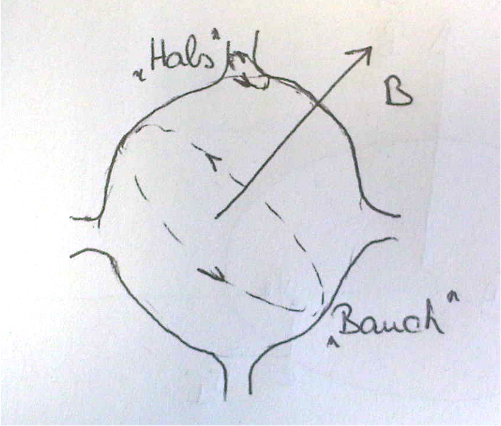
\includegraphics[width=0.75\textwidth]{kap10_07.png}


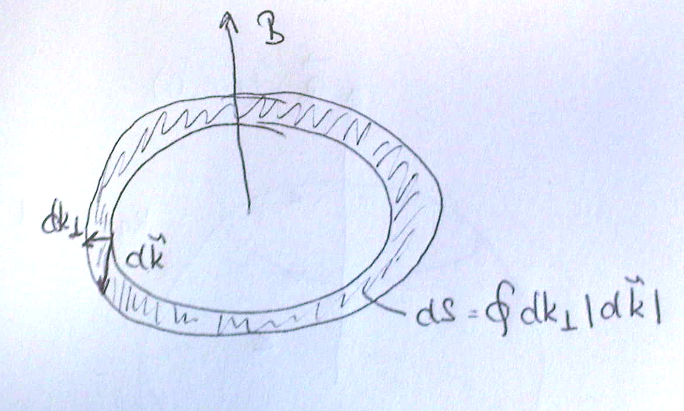
\includegraphics[width=0.75\textwidth]{kap10_08.png}


\[dS = \oint dk_\bot |dk|\]

für freien \(e^-\)-nen: \(\omega_c = \frac{eB}{m}\); \(T_c = \frac{2\pi m}{eB}\); \(\frac{dS}{\partial E}= \frac{2\pi m}{\hbar^2}\): Bloch Elektronen \(\boxed{m\equiv m_c}\)

\section{Experimentelle Methoden zur Bestimmung der Fermi-Flächen}

\begin{enumerate}
\item[1)] de-Haas-van-Alphen-Oszillationen (Magnetisierung)
\item[2)] Schubnikov-de-Haas-Oszillationen (Wiederstand)
\item[3)] Zyklotronresonanz: Gantmacher-Effekt
\end{enumerate}
 
Landau-Niveaus: Quantisierung der Elektonbahnen im Magnetfel (1930)

\[\frac{1}{2m}(-i\hbar\nabla + e\vec A)^2\psi = E\psi\]

Coulomb-Eichung \(\vec A = (0,xB,0)\)
Landau-Eichung \(\vec A = (-yB,0,0)\) oder \(-\frac{yB}{y},\frac{xB}{2},0\)

Eigenwerte: \(E = E_l  + E(k_z) = (l+\frac{1}{2})\hbar\omega_c+\frac{\hbar^2k^2_z}{2m}\) mit \(l\) als Quantenzahl

Landau-Röhren (Zilinderoberflächen im \(\vec k\)-Raum): \(\frac{\hbar^2(k^2_x+k^2_y}{2m}\)

\[\sqrt{k^2_x+k^2_y}=\left[\frac{2m}{\hbar}(l+\frac{1}{2})\omega_c\right]^{\frac{1}{2}} = \left[ \frac{2eB}{\hbar}(l+\frac{1}{2}\right]^{\frac{1}{2}}; \Rightarrow r_l=\left[(l+\frac{1}{2})\frac{2\hbar}{eB}\right]^{\frac{1}{2}}\]

\(k \Leftrightarrow r \) Faktor \(\frac{\hbar}{eB}\)


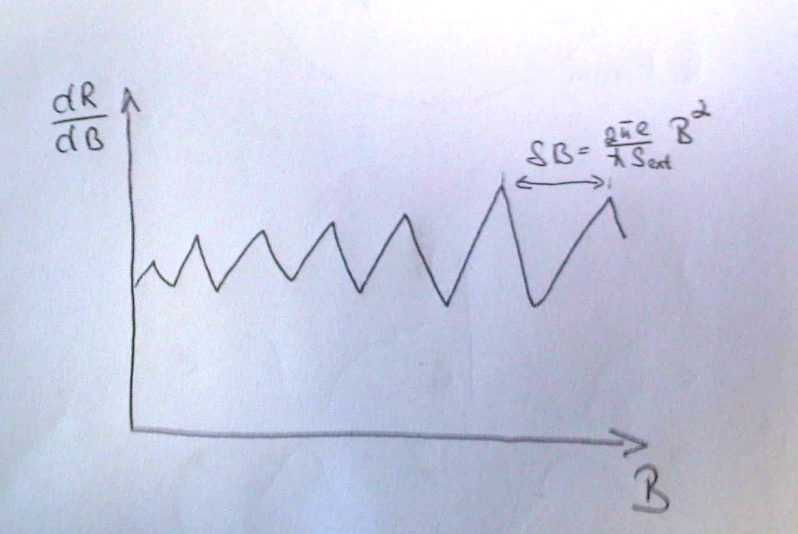
\includegraphics[width=0.75\textwidth]{kap10_09.png}

\[\delta B = \frac{2\pi e}{\hbar S_ext}B^2\]

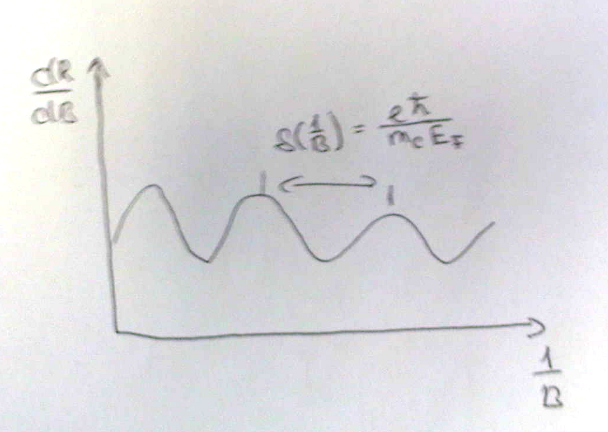
\includegraphics[width=0.75\textwidth]{kap10_10.png}

\[\delta \frac{1}{B} = \frac{e\hbar}{m_c E_F}\]

